\documentclass{article}

\usepackage{graphicx}
\usepackage{tikz}
\usepackage{tikzsymbols}
\usetikzlibrary{calc,patterns,shapes.geometric}
\pagestyle{empty}
\usepackage[margin=0pt]{geometry}
\geometry{papersize={14in,12in}}

\def\centerarc[#1](#2)(#3:#4:#5){\draw[#1] ($(#2)+({#5*cos(#3)},{#5*sin(#3)})$) arc (#3:#4:#5);}

\begin{document}
	\begin{figure}
		\centering
		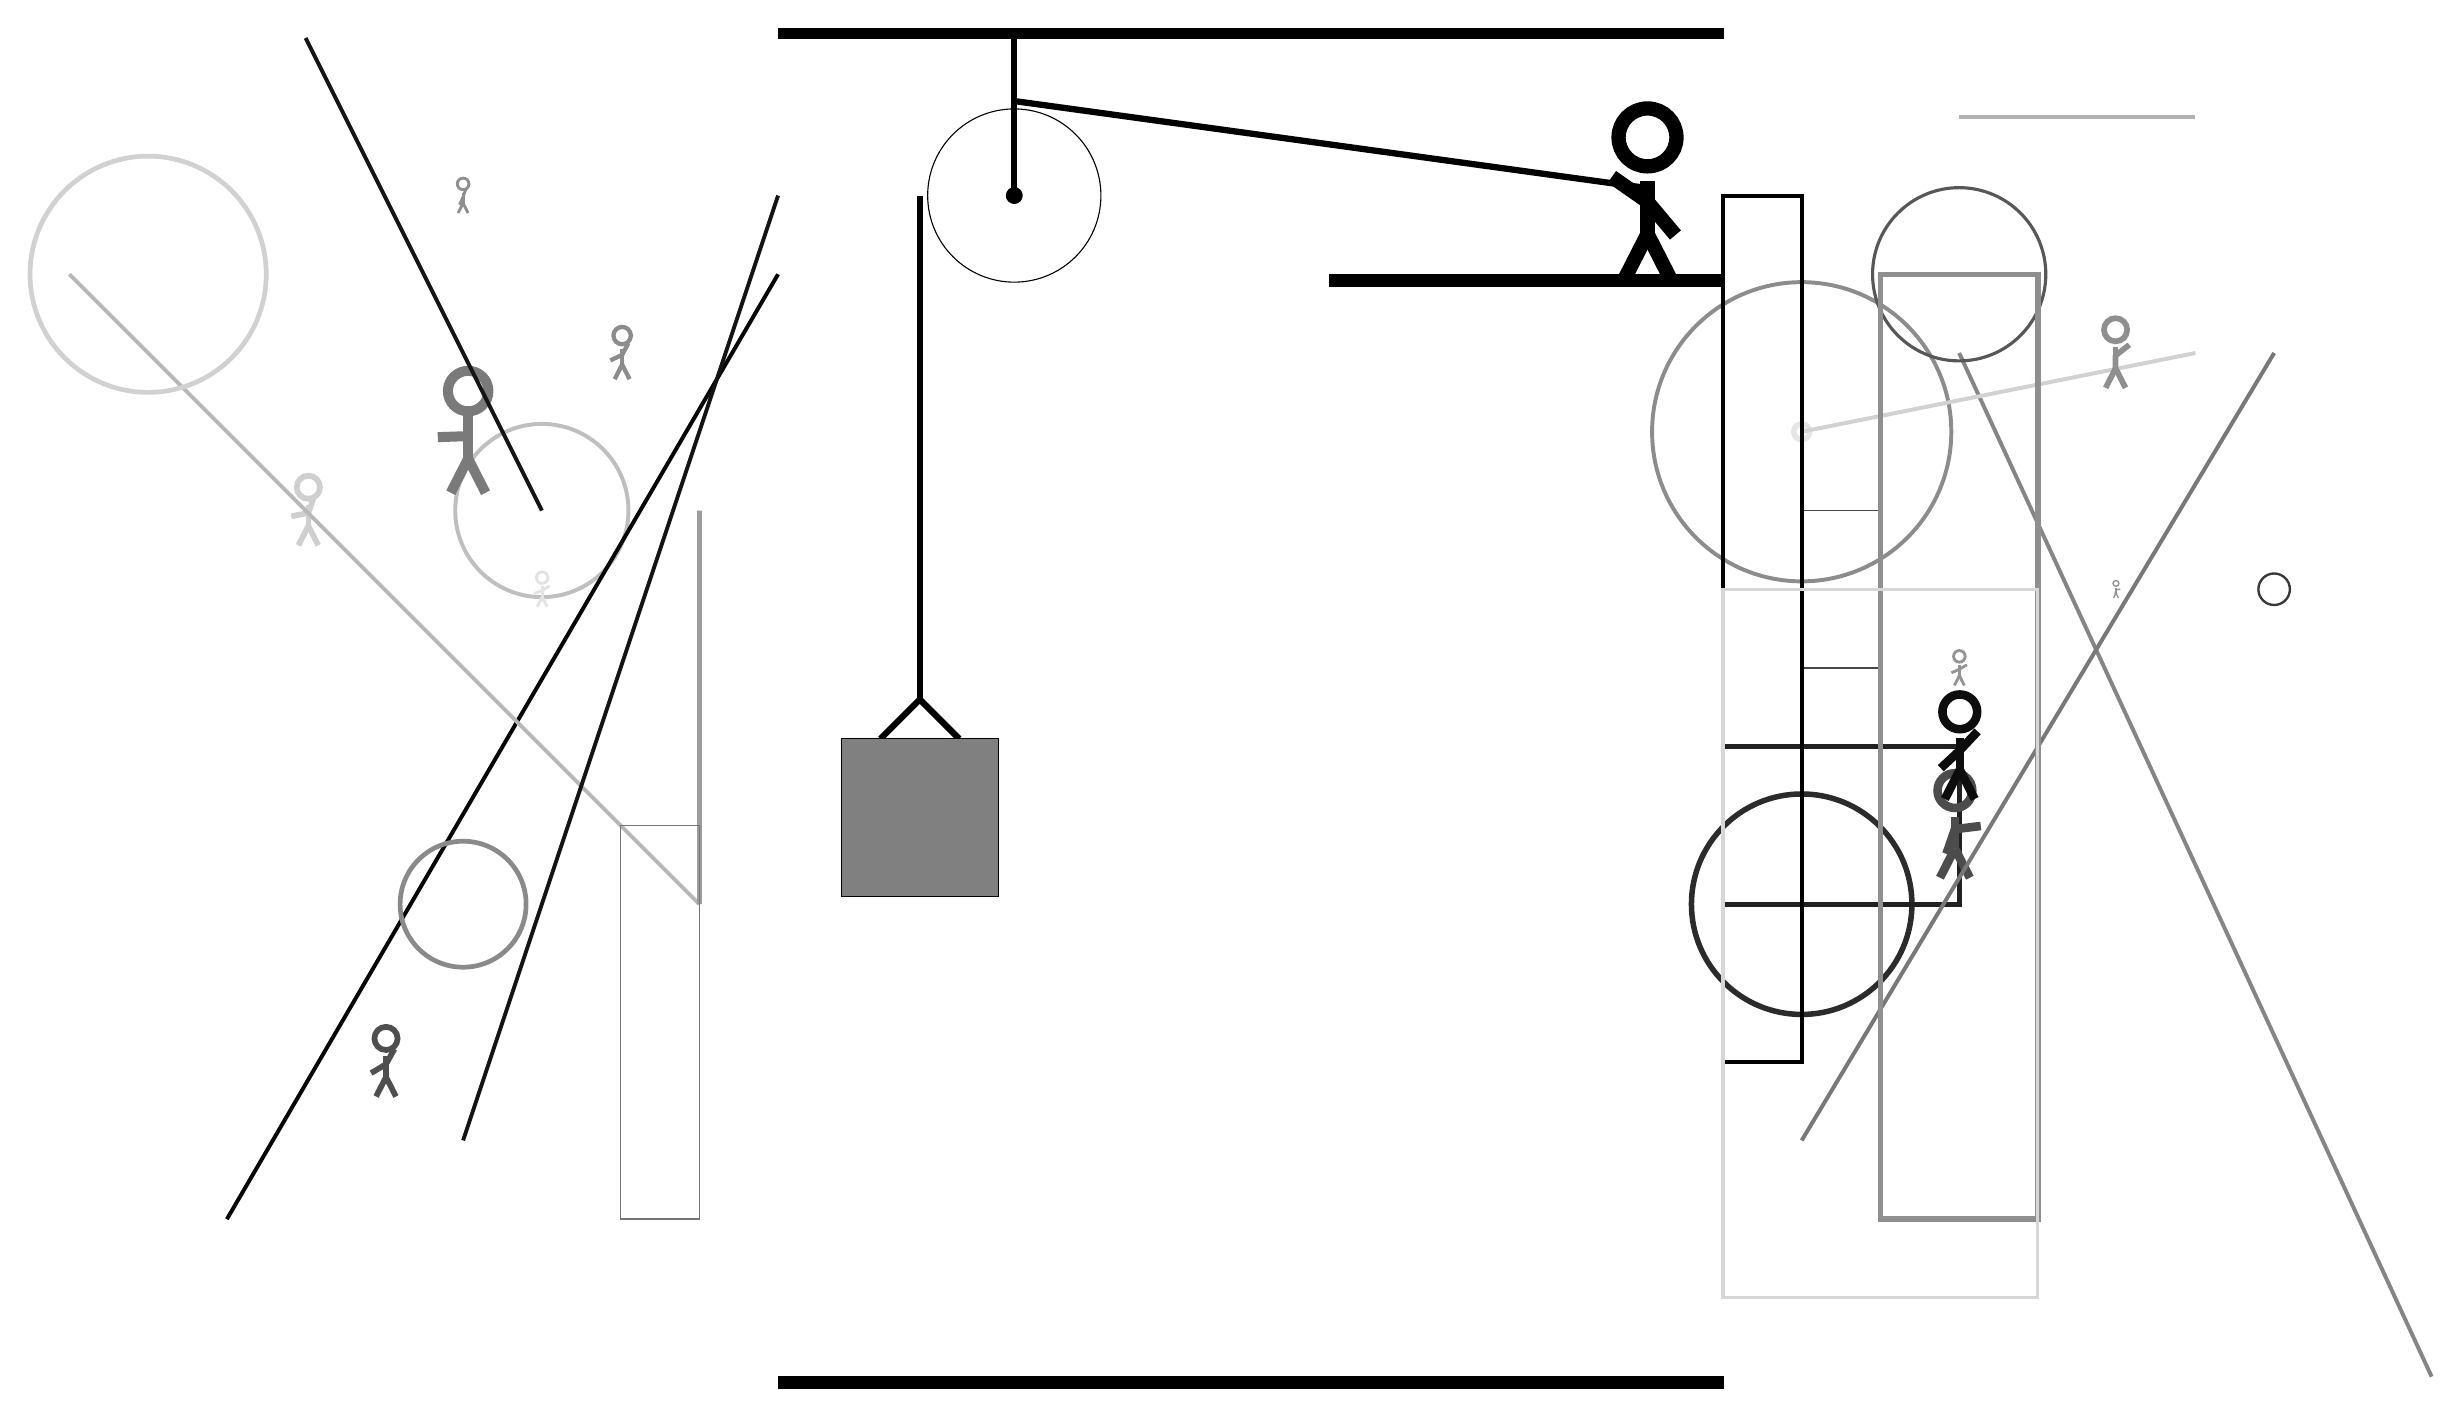
\begin{tikzpicture}
			%%%%% START %%%%%
			
			\draw[fill=black] (-2, 14) rectangle (10, 14.125);
			
			\draw (1, 12) circle (1.1);
			\draw[fill=black] (1, 12) circle (0.1);
			\draw[line width=0.8mm] (1, 14) -- (1, 12);
			
			\draw[line width=0.8mm](-0.7, 5.1) --  (-0.2, 5.6) -- (0.3, 5.1);
			\draw[fill=black!50] (-1.2, 5.1) rectangle (0.8, 3.1);
			
			\draw[line width=0.8mm](-0.2, 12) -- (-0.2, 5.6);
			\centerarc[line width=0.8mm](1, 12)(90:180:1.2000000000000002)
			\draw[line width=0.8mm](1, 13.2) -- (9, 12.1);
			
			\draw [line width=0.5mm, color=black!25](-5, 8) circle (1.1);
			
			\draw[line width=0.2mm, color=black!72] (11, 8) rectangle (12, 6);
			\draw[line width=0.5mm, color=black!48](13, 10) -- (19, -3);
			\draw[line width=0.5mm, color=black!98](-2, 11) -- (-9, -1);
			\node[line width=0.4mm, color=black!11] at (-5, 7) {\Strichmaxerl[2][21][32]};
			\node[line width=0.3mm, color=black!19] at (-8, 8) {\Strichmaxerl[4][11][71]};
			
			\draw [line width=0.3mm, color=black!78](17, 7) circle (0.2);
			\draw[line width=0.5mm, color=black!28](-3, 3) -- (-11, 11);
			\draw [line width=0.7mm, color=black!83](11, 3) circle (1.4);
			\draw [line width=0.5mm, color=black!45](11, 9) circle (1.9);
			\draw [line width=0.6mm, color=black!46](-6, 3) circle (0.8);
			
			\draw[line width=0.6mm, color=black!87] (10, 3) rectangle (13, 5);
			\draw [line width=0.7mm, color=black!10](11, 9) circle (0.1);
			
			\draw[line width=0.5mm, color=black!92](-6, 0) -- (-2, 12);
			\node[line width=0.5mm, color=black!70] at (13, 4) {\Strichmaxerl[6][71][7]};
			\node[line width=0.4mm, color=black!44] at (-6, 12) {\Strichmaxerl[2][66][70]};
			
			\node[line width=0.7mm, color=black!42] at (15, 7) {\Strichmaxerl[1][78][10]};
			\draw [line width=0.6mm, color=black!18](-10, 11) circle (1.5);
			\draw [line width=0.5mm, color=black!67](-4, 5) circle (0.0);
			\node[line width=0.7mm, color=black!52] at (-6, 9) {\Strichmaxerl[7][2][90]};
			\node[line width=0.2mm, color=black!69] at (-7, 1) {\Strichmaxerl[4][31][61]};
			
			\draw [line width=0.4mm, color=black!66](13, 11) circle (1.1);
			
			\draw[line width=0.5mm, color=black!53](11, 0) -- (17, 10);
			\draw[line width=0.5mm, color=black!18](11, 9) -- (16, 10);
			\draw[line width=0.5mm, color=black!92](-5, 8) -- (-8, 14);
			
			\draw[line width=0.7mm, color=black!39] (-3, 8) rectangle (-3, 3);
			\node[line width=0.7mm, color=black!44] at (15, 10) {\Strichmaxerl[4][89][38]};
			\draw[line width=0.2mm, color=black!54] (-4, 4) rectangle (-3, -1);
			\draw[line width=0.5mm, color=black!30](13, 13) -- (16, 13);
			\draw[line width=0.7mm, color=black!44] (12, 11) rectangle (14, -1);
			\draw[line width=0.5mm, color=black!100] (10, 12) rectangle (11, 1);
			
			\node[line width=0.4mm, color=black!45] at (-4, 10) {\Strichmaxerl[3][25][62]};
			\draw[line width=0.4mm, color=black!16] (10, 7) rectangle (14, -2);
			\node[line width=0.3mm, color=black!42] at (13, 6) {\Strichmaxerl[2][24][30]};
			\node[line width=0.5mm, color=black!95] at (13, 5) {\Strichmaxerl[6][43][47]};
			
			\node at (9, 12) {\Strichmaxerl[10][-35][-50]};
			\draw[fill=black] (5, 11) rectangle (10, 10.85);
			
			\draw[fill=black] (-2, -3) rectangle (10, -3.15);
			
			%%%%% END %%%%%
		\end{tikzpicture}
	\end{figure}	
\end{document}